% textidote: ignore begin
\section{Existing solutions and their operational mechanisms}\label{sec:extant-solutions-and-their-operational-mechanisms}
% textidote: ignore end

Commuting is one of the staples, so to speak, of modern life, and a central part of the post-modern industrialized
society.
As cities rapidly grew after the industrial revolution and more and more large-scale workplaces became the norm in
cities, people started commuting to work from suburban areas to the city as mentioned earlier.

This question especially became relevant in recent times due to the increasingly noticeable effects of climate change
and the scientific evidence that increased \unit{CO_{2}} emissions greatly contribute to climate change.
Other questions the modern-day commuter might ask themselves are: Do I need/want to commute every day, or is it ok if I
work from home part of the week?
What should be the balance between cost and environmental protection?
Do I live in an area where the availability of public means of transportation is scarce, so I am more inclined to use a
car?
One of the simpler questions someone that considers commuting could ask themselves is merely: What commuting route
should I choose?
With the advent of the digital age and smartphones, the answer to this question have become commuting planner
applications, that have become increasingly popular in recent years, helping individuals plan their daily commutes
efficiently and minimize travel-related stress.
These applications offer various features and functionalities, but they often have shortcomings that prevent the
commuter from more advanced planning strategies, including the lack of easy access to cost and environmental impact
information, e.g., how much \unit{CO_{2}} will be spent on a trip, how much a trip will cost, as well as limited user
control over how these factors are weighed in route calculations.
Existing solutions include the (mostly) worldwide available Google Maps, the popular Danish Rejseplanen service and a
couple of other mobile and web applications that are not location-bound but can be used internationally, like
\url{https://commute.org/}.
We will now look at some existing solutions and discuss their shortcomings to better understand the root of the problem.

% textidote: ignore begin
\subsection{Google Maps}\label{subsec:google-maps}
% textidote: ignore end

\begin{figure}
    \centering
    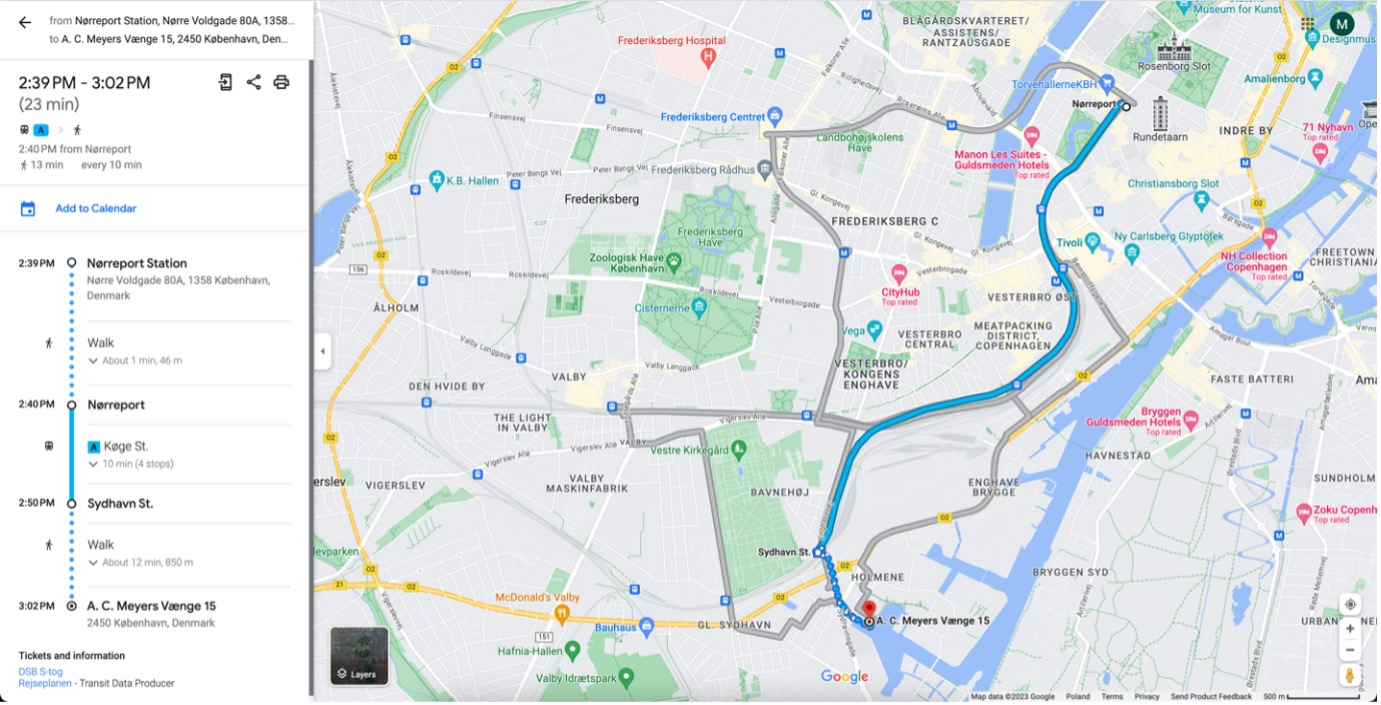
\includegraphics[width=\textwidth]{google-maps}
    \caption{Google Maps web UI.}
    \label{fig:figure6}
\end{figure}

Google Maps is another online service used for travelling.
It is one of the most extensive and detailed mapping databases globally.
Its comprehensive coverage includes even remote areas, making it a go to for travelers and commuters.
Whether you're navigating in unknown areas or exploring remote landmarks, Google Maps is sure to provide accurate
mapping data~\cite{googlemaps2023}.

\subsubsection{Usage}\label{subsubsec:usage}

The above-mentioned application is a widely used travel and commuting planner that provides detailed navigation and
route information and can also be seen in Figure~\ref{fig:figure6}.
While it offers estimated travel time and distance, it lacks a direct and user-friendly way to determine the cost of the
trip or the \unit{CO_{2}} footprint.
Users cannot easily access information about how much money the trip will cost, as Google Maps does not integrate with
financial or payment apps to calculate expenses like tolls, fuel, or public transportation fees.
This makes sense since Google tries to target a large international audience with the application, making is difficult
or nearly impossible to cover every localized payment solution or traveling restriction.
Similarly, it does not provide real-time data on the \unit{CO_{2}} emissions associated with the chosen route, making it
challenging for users to make informed decisions about their environmental impact.

\begin{wrapfigure}{l}{0.5\textwidth}
    \begin{center}
        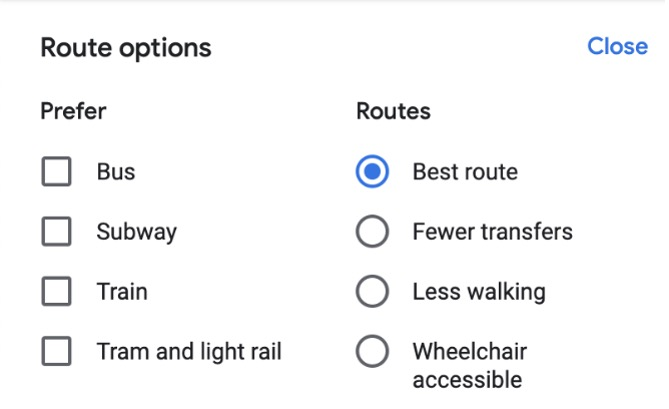
\includegraphics[width=0.4\textwidth]{google-maps-options}
    \end{center}
    \caption{Google Maps web UI options.}
    \label{fig:figure7}
\end{wrapfigure}

Users have very limited control over how cost and environmental factors are weighed in route calculations, as Google
Maps primarily focuses on travel time and distance.
The only available selection options, as can be seen in Figure~\ref{fig:figure7}, are preferences for means of
transportation and whether the route should be calculated with ``fewer transfers'', ``less walking'' or ``wheelchair
accessible'', where all three of the options seem to be tailored towards people with restricted mobility.

% textidote: ignore begin
\subsubsection{Ongoing developments}\label{subsec:ongoing-developments}
% textidote: ignore end

Google Maps continues to evolve with regular updates and new features.
Recent advancements include enhanced AR (Augmented Reality) navigation, which overlays digital information onto
a real-world environment through the user's smartphone camera.
With Augmented Reality navigation you would be able to see the navigation through your smartphone when holding it
vertically. \cite{googlemapsAR2023}

% textidote: ignore begin
\subsection{Rejseplanen}\label{subsec:rejseplanen}
% textidote: ignore end

In Denmark, the most popular commuting planner application by far is Rejseplanen.
This application, just like Google Maps, is both available as a web and mobile application.
The app lets the traveler or commuter to enter trip starting and ending locations, which it then uses to calculate a
route using public means of transportation or as secondary options as walking routes.
When a route is calculated, the user is presented with a list-like interface from which the details of the trip can be
read; what means of transportation will be used, which lines, what the departure and arrival times are, and if there are
any special restrictions on the trip.
See Figure~\ref{fig:figure8}.

\begin{wrapfigure}{r}{0.4\textwidth}
    \begin{center}
        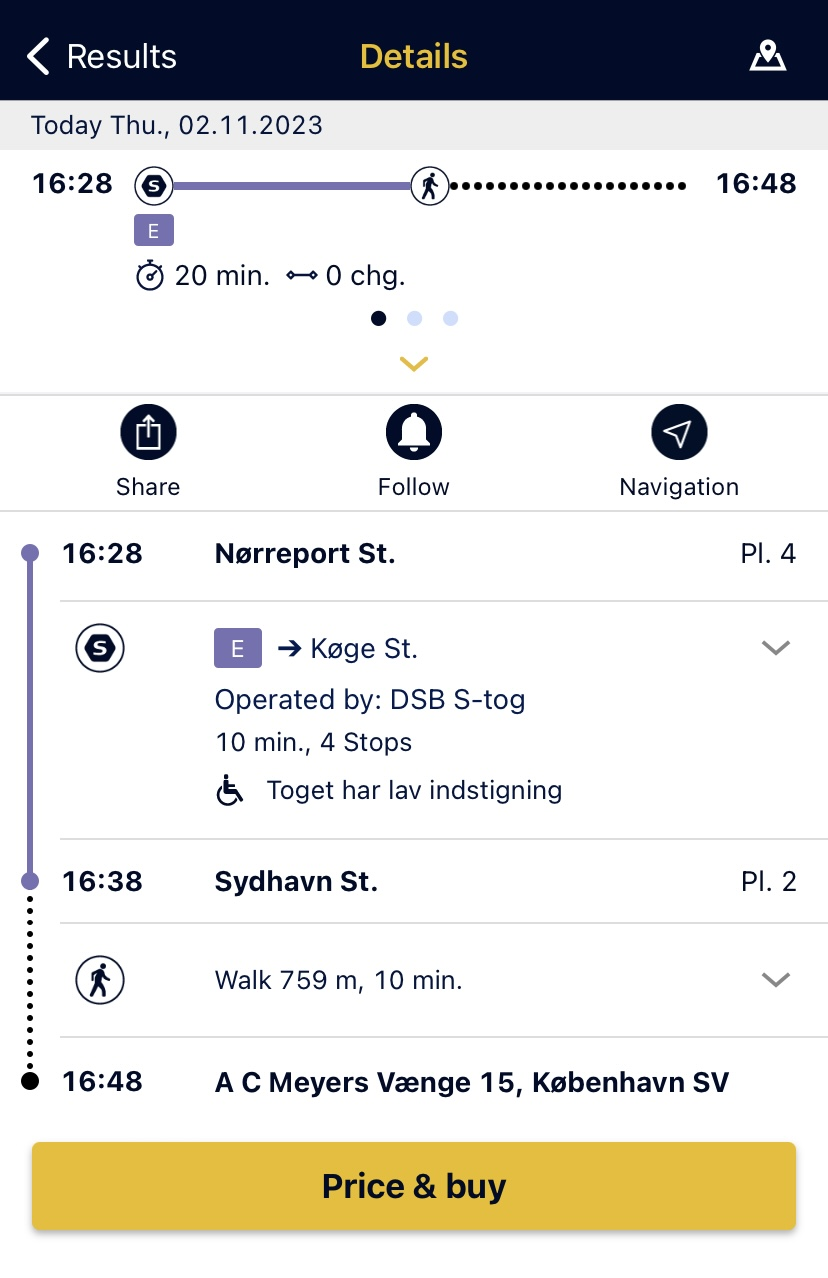
\includegraphics[width=0.3\textwidth]{rejseplanen-trip}
    \end{center}
    \caption{Rejseplanen mobile UI trip planner.}
    \label{fig:figure8}
\end{wrapfigure}

With ``Rejseplanen'', you can input your departure point and destination point to get information about the fastest,
cheapest or most convenient way to travel from point A to B using public transport.
The service provides detailed information about the departure times, transfers, expected arrival times and prices.
It also provides any additional information about the delays or canceled departures in the operation of public
transport~\cite{rejseplanen2023}.

Rejseplanen also supports ticket purchases for public transportation but ``Rejseplanen'' itself does not sell tickets
directly.
Instead, it redirects you to another website or dedicated app DOT (if installed) associated with the respective
transportation service provider.
The redirection ensures a smooth and integrated ticketing experience, allowing the users to complete their journey
planning and ticket purchase in a cohesive manner~\cite{rejseplanen2023}.

Getting the price of the trip is possible too, but in a primitive manner that doesn't consider factors such as if the
user is a tourist or a regular resident, which is an important feature since tourists might have different traveling
strategies than regular residents, and additionally tourists might not use the prepaid Rejsekort card, etc.
There is an additional option of adding your Rejsekort ID to the app, so it can calculate the trip price based on your
card plan, but even that feature is kept rather simple, possibly because the Danish transportation authorities also
released the DOT app, whose primary responsibility is exactly that: calculating trip prices and buying tickets.
See Figure~\ref{fig:figure9}.

\begin{figure}
    \centering
    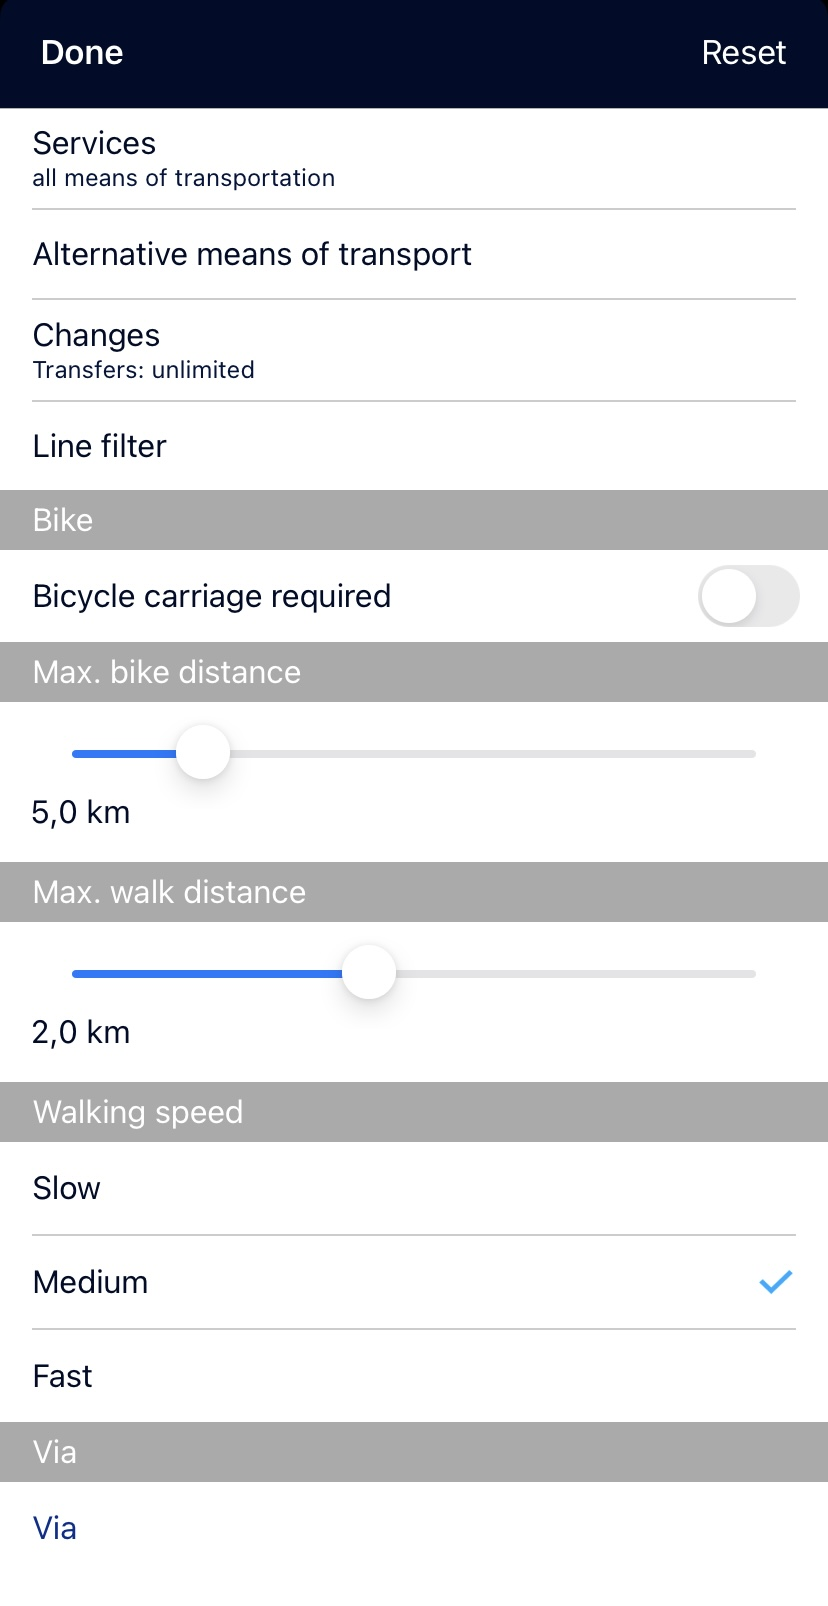
\includegraphics[width=0.5\textwidth]{rejseplanen-options}
    \caption{Rejseplanen mobile UI trip planner options.}
    \label{fig:figure9}
\end{figure}

The user can also customize the trip's parameters slightly, e.g., if it's a biking or a walking trip, what the maximum
allowed biking or walking distance should be, whether the user is a ``slow'', ``medium'' or ``fast'' walker (even though
there is no guideline for how fast exactly each of these options is), and a few additional details, but a feature that
definitely lacks is the calculation of the trip’s total \unit{CO_{2}} emissions, which is an important factor in the
modern-day world.

\subsubsection{What makes rejseplanen great?}
\begin{itemize}
    \item \textbf{Comprehensive data integration}: Rejseplanen integrates data from various transportation providers,
    thus ensuring up-to-date and accurate information.
    \item \textbf{Very efficient}: Rejseplanen provides a quick and convenient travel plan, saving time for daily
    commuters.
    \item \textbf{User-friendly}: Rejseplanen provides additional features such as filtering out specific trains or
    buses, so your route matches your personal preferences and enhancing the user experience.
\end{itemize}

In summary, ``Rejseplanen'' serves as an indispensable tool for individuals navigating Denmark's public transport system
offering a solution for journey planning, real-time updates and ticket purchases, contributing to the overall efficiency
and convenience of public transportation for commuters in the country.

% textidote: ignore begin
\subsubsection{Data sources for Rejseplanen}
% textidote: ignore end

Rejseplanen is jointly owned by DSB, Movia, Metroselskabet, NT, Midttrafik, Sydtrafik, Fynbus, and BAT\@.
As a result of its ownership by these various transportation service providers, Rejseplanen has access to the data
necessary to determine the most efficient public transport routes~\cite{rejseplanen2023}.

Rejseplanen's effectiveness in providing accurate and up-to-date public transport information is directly linked to its
access to a diverse range of data sources.
The ownership structure, with contributions from major transportation service providers in Denmark, ensures a
comprehensive and collaborative approach to gathering the necessary data for efficient journey planning.

By drawing data from these diverse data sources, ``Rejseplanen'' ensures a holistic approach to journey planning,
covering various modes of transportation and providing users with accurate, timely and relevant information for their
public transport needs.

\subsection{Apple Maps}\label{subsec:apple-maps}

The software already mentioned are two of the most important software for personal transportation.
Rejseplanen specifically focused on Denmark and Google Maps which is focussed around the whole globe.
Another software which has some of the same capabilities is Apple Maps.

Apple Maps is mostly the same as Google Maps, it also has very detailed mapping data.
Apple Maps also provides navigation function like Google Maps that is with turn-by-turn directions for driving, walking
and public transportation.
It also supports real-time traffic information and alternative routes to help users reach their destination more
efficiently.
Apple Maps can provide various information about shopping centers, restaurants, hotels and gas stations.
Some of that information includes user reviews, photos, contact details and hours of operation.
Google Maps does also provide this kind of information.

Google Maps used to be the default web mapping service for iOS, but they replaced Google Maps with their own version
which is of course Apple Maps now~\cite{applemaps2023}.

